\chapter*{Introduction}\label{chap:intro}
\addcontentsline{toc}{chapter}{Introduction} % ensures it appears in the main TOC
\mtcaddchapter
\markboth{INTRODUCTION}{INTRODUCTION} % <-- fixes header marks


\section*{Historical background}
\addcontentsline{toc}{section}{Historical background} % ensures it appears in the main TOC


The field of quantum optomechanics investigates the interaction between light and the motion of mechanical resonators, which can take many forms: radiation-pressure induced displacements, thermally driven vibrations, quantum zero-point fluctuations, etc. The generic optomechanical system consists in an optical cavity with a moving mirror (Fig. \ref{fig:cavitiesOM}.(a)): photons can change the resonator dynamics (via radiation pressure, photothermal effects, etc.), and conversely, the motion of the mechanical element modifies the cavity optical field. Measuring the output optical field thereby provides information about the mechanical motion and/or the environment it is coupled to, while appropriately engineering the input optical field enables control of the resonator dynamics. The crucial question that arises for both mechanical motion readout and control is: what are the fundamental limits imposed by quantum mechanics? \\

% \begingroup
% \renewcommand{\thefigure}{\arabic{figure}} % only 1,2,3... (no chapter)
% \begin{figure}[t]
%   \centering
%   \includegraphics[width=\linewidth]{...}
%   \caption{...}
%   \label{fig:myfig}
% \end{figure}
% \endgroup


In the context of gravitational wave interferometers (GWI), where the idea is to measure the differential changes in length of two orthogonal km-scale optical cavities induced by passing gravitational waves, it was realized in the 1970s that the sensitivity of such interferometers was ultimately limited by quantum fluctuations of the input light field \cite{Braginsky1968JETP_ClassicalQuantumRestrictions,Caves1980PRL_RadiationPressureFluctuations}. It was soon understood that these limitations were ubiquitous in optomechanical systems, setting fundamental bounds to the sensitivity of position measurements of mechanical resonators, from nano- to macroscopic scales. The quantum nature of light imposes two contributions: shot-noise, arising from the intrinsic phase fluctuations of the optical field, and radiation-pressure noise, arising from the optical field amplitude fluctuations driving the mechanical resonator i.e. the cavity mirror, and translating into an extra phase noise contribution in the detected optical field. These two contributions trade-off against each other, leading to an ultimate sensitivity known as the Standard Quantum Limit (SQL) \cite{BraginskyVorontsovThorne1980Science_QND,BraginskyKhalili1992Book_QuantumMeasurement, clerk_introduction_2010}. It was then proposed to inject squeezed states of light into the interferometer dark port to reduce quantum noise and improve sensitivity beyond the SQL \cite{caves1981}. On the experimental side, while the shot-noise has been observed in optical interferometers since the 1980s \cite{Loudon1983QuantumTheoryOfLight}, the radiation-pressure noise has however proven very challenging to observe experimentally, as it competes with thermal noise effects which usually dominate for micro-scale mechanical resonators, even at cryogenic temperatures. \\ 

Experimental \textit{tabletop} optomechanics then truly kicked off in the mid 1990s, when stable laser sources, low-loss optical coatings, quantum-limited detection setups and high-Q mm-scale mechanical resonators became available. The idea at the time was to take advantage of the smaller mass of the resonators (compared to the kg-scale of GWI mirrors) to (actually, not so) easily demonstrate the effect of quantum fluctuations of radiation pressure upon the motion of the moving mirror. Notable milestones include the demonstration of feedback cooling of mechanical resonators in 1999 \cite{cohadon_cooling_1999}, radiation pressure cooling in 2006 \cite{arcizet2006,Gigan2006}, the observation of strong optomechanical coupling in 2009 \cite{groblacher2009}, ground state cooling in 2011 \cite{Teufel2011}, and the direct observation of radiation-pressure noise in a micro-optomechanical system in 2013 \cite{regal2013}. \\ 

\begingroup
\renewcommand{\thefigure}{\arabic{figure}} % only 1,2,3... (no chapter)
\begin{figure}
\centering
\includegraphics[width=\textwidth]{./chap1/fig/cavitiesOM_MIM.pdf}
\caption{ Optomechanical cavities with a moving end-mirror modelled as a spring (a) and a membrane based optomechanical system (b). While the moving-mirror cavity is the simplest optomechanical system, it requires to optimize both the optical and mechanical properties of the end-mirror simultaneously, which can be challenging. The membrane systems, on the other hand, separates the optical and mechanical design constraints, enabling the use of high-finesse cavities with low-loss mechanical resonators embedded within. } 
\label{fig:cavitiesOM}
\end{figure}
\endgroup



Present research in quantum optomechanics now focus on broad range of topics, that we can loosely put in four main categories: (i) the study of quantum limits in position measurements; (ii) the development of improved optomechanical sensors; (iii) the investigation of the fundamental quantum physics of the mechanical degree of freedom; and (iv) applications to quantum information. These topics all take advantage of the versatility of optomechanical systems, than can be coupled to a large spectrum of systems, such as laser and microwave light, electric and magnetic fields, two-level systems (spins, color centers...), acceleration and forces, etc. 

\begingroup
\renewcommand{\thefigure}{\arabic{figure}} % only 1,2,3... (no chapter)

\begin{figure}
\centering
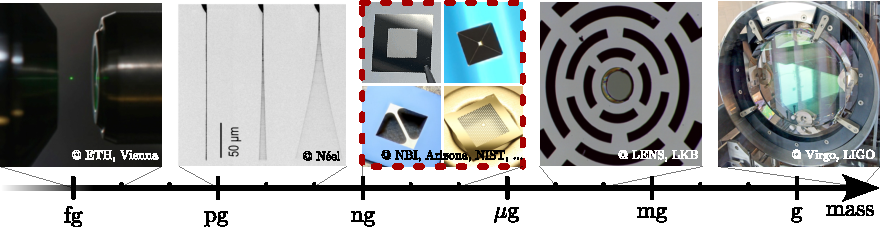
\includegraphics[width=\textwidth]{./chap1/fig/resonatorsfamily.pdf}
\caption{Non-exhaustive overview of mechanical resonators used in free-space optomechanics experiments. From left to right: a fg-scale nanosphere levitated with an optical tweezer \cite{Delic2020}, a pg-scale nanowire \cite{Fogliano2021}, ng-scale membrane based resonators (plane membranes, a trampoline resonator, a strip and a phononic crystal membrane) \cite{Norcada_QuantumStandardDevices,Wilson2024, Hyatt2025, Tsaturyan2017}, a $\mu$g-scale \textit{wheel} resonator \cite{Marin2015} and a Virgo/LIGO like kg-scale mirror \cite{Degallaix2023}. The diversity of mechanical resonators used in optomechanics experiments is a testament to the versatility of the field, where the mechanical element can be tailored to the specific application at hand. The red frame highlights the variety of membrane based resonators that can be used in membrane-in-the-middle or membrane-at-the-end optomechanical systems. }
\label{fig:resonatorsfamily}
\end{figure}
\endgroup

\section*{Relevance of this work}
\addcontentsline{toc}{section}{Relevance of this work} % ensures it appears in the main TOC
This thesis belongs to the first category of research mentioned above, where we focus on the use and manipulation of squeezed light to improve the measurement sensitivity beyond the SQL. We do so by leveraging two main experimental ingredients:
\begin{itemize}
    \item \textbf{Membrane based optomechanical systems} as tunable optomechanical platforms. (Chap. II and IV)
    \item \textbf{Frequency-dependent squeezed light} as a sub-SQL probe (Chap. II and V) 
\end{itemize}

\noindent \textbf{Membrane based optomechanical systems:} Membrane-based optomechanical systems consist of a thin dielectric membrane placed inside an optical cavity, forming a so-called "membrane-in-the-middle" (MIM) or "membrane-at-the-end" (MATE) configuration \cite{Thompson2008Nature,Jayich2008NJP}. We show a generic view of a membrane based system in Fig. \ref{fig:cavitiesOM}.(b). Introduced in 2008, the MIM architecture has become a popular platform for optomechanics. The smart workaround of using a thin membrane as the mechanical resonator, rather than a moving end-mirror, enables the use of high-finesse cavities with low mechanical loss resonators embedded within, hence splitting the optical and mechanical design constraints. This has led to numerous experimental demonstrations, including approaching the membrane ground state from room temperature \cite{Saarinen23}, strong light mediated coupling between a membrane and a spin \cite{science.abb0328}, state transfer between light and mechanics \cite{PhysRevLett.132.100802}, and membrane assisted squeezing generation \cite{PhysRevX.3.031012, Kippenberg_2024}. Other advantages of such systems include the ability to interchange easily the membrane resonator, enabling the exploration of a wide variety of mechanical resonators (red frame of Fig. \ref{fig:resonatorsfamily}), and the tunability of various parameters and couplings to explore a wide range of optomechanical phenomena. \\

The MATE configuration, however, remains less explored compared to the MIM configuration, with only a handful of experimental realizations reported in the literature \cite{Dumont:19}. The MATE/MIM geometries display appealing features, such as a large linear coupling range, quadratic points, and greater tunability than standard moving-mirror cavities, making them promising candidates for future optomechanical experiments. \\

\noindent \textbf{Frequency-dependent squeezed light:} Squeezed states of light are non-classical states where the quantum fluctuations of one quadrature (amplitude or phase) are reduced below the vacuum level, at the expense of increased fluctuations in the orthogonal quadrature, by virtue of the Heisenberg inequality. Experimentally demonstrated in 1985 \cite{slusher1985squeezed}, squeezed light has since then found applications in quantum information, quantum metrology and fundamental tests of quantum mechanics. In the context of optomechanical measurements, squeezed light can be used to reduce quantum noise and improve sensitivity beyond the SQL \cite{caves1981}. However, due to the trade-off between shot-noise and radiation-pressure noise, frequency-independent squeezed light can only improve sensitivity in a limited frequency band. To achieve broadband sensitivity improvement, it is necessary to use frequency-dependent squeezed light, where the squeezing angle rotates as a function of frequency \cite{klmtv}, and where the frequency range over which the squeezing angle rotates is to be tuned to a specific mechanical resonator, from kg-scale GWI mirrors to ng-scale micro-resonators. The implementation of frequency-dependent squeezing has been a major milestone in the field, with recent demonstrations in GWIs \cite{ Virgo2023, LIGO2020}. \\


With a few experimental demonstrations of frequency-independent squeezing injection in micro/nano-scale optomechanical systems reported in the literature over the past ten years \cite{hoff2013_quantumEnhancedMicromechanical, schafermeier2016_quantumEnhancedFeedbackCooling, clark2016_observationStrongRadiationPressure,li2018_quantumEnhancedOptomechanicalMagnetometry, xia2023_entanglementEnhancedOptomechanicalSensing, Schnabel2020, Yap2020}, tabletop frequency-dependent squeezing, however, is yet to be routinely injected in mm-scale optomechanical systems. This thesis contributes to this emerging field by presenting the steps toward the development of a frequency-dependent squeezed light source tailored for MHz-frequency membrane-based optomechanical systems. \\ 



All in all, even fewer (if no) research projects have combined both frequency-dependent squeezed light and membrane-based optomechanical systems. This thesis thus aims at bridging this gap by developing the experimental tools necessary to implement frequency-dependent squeezing in a MATE optomechanical cavity, with the long-term goal of demonstrating broadband sub-SQL measurements in such systems. A particular attention is given to the afforfability and versatility of the developed experimental methods by detailing the use of open-source hardware and software solutions. Additionally, this manuscript details the theory of squeezed light optomechanics in depth, and provides various key equations and numerical tools that can be used to model quantum noise in realistic optomechanical systems.

\section*{Thesis outline}
\addcontentsline{toc}{section}{Thesis outline} % ensures it appears in the main TOC
 


\noindent \textbf{Chapter I} presents the theoretical background required to motivate and discuss the experiments reported in this manuscript: the optical field (classical spatial-mode description, classical modulations used for sensing and locking, and quantum treatment), Fabry–Perot cavities as the workhorse of the experimental platforms, and the main detection schemes. \\ 

\noindent \textbf{Chapter II} introduces squeezed light and the mechanical response of a mirror to radiation-pressure forces, establishing the Standard Quantum Limit and motivating squeezed-light injection to improve displacement sensitivity; both QSN and QRPN are discussed, together with numerical tools used to compute noise spectra in realistic situations. It also presents the specific properties of membrane-based optomechanical systems, focusing on the MATE configuration. \\ 

\noindent \textbf{Chapter III} provides an overview of the experimental methods developed throughout my PhD work, with emphasis on locking and detection techniques largely implemented within the PyRPL architecture. \\

\noindent \textbf{Chapter IV} focuses on the MATE cavity geometry used to realize a moving-mirror cavity, including the motivation for this approach, the experimental characterization of early prototypes, and design considerations for a cryogenic MATE cavity incorporating a SiN membrane resonator. \\ 

\noindent \textbf{Chapter V} describes the development, upgrade and characterization of the squeezed-light source, detailing its layout and operation, presenting preliminary squeezing results, and briefly outlining the work carried out in 2023 on the Advanced Virgo squeezing filter cavity.  \\

\noindent The manuscript concludes with a summary of the experimental results and perspectives toward a broadband demonstration of sub-SQL measurements.